\documentclass{article}

\usepackage{graphicx}
\usepackage{tikz}
\usepackage{tikzsymbols}
\usetikzlibrary{calc,patterns,shapes.geometric}
\pagestyle{empty}
\usepackage[margin=0pt]{geometry}
\geometry{papersize={14in,12in}}

\def\centerarc[#1](#2)(#3:#4:#5){\draw[#1] ($(#2)+({#5*cos(#3)},{#5*sin(#3)})$) arc (#3:#4:#5);}

\begin{document}
	\begin{figure}
		\centering
		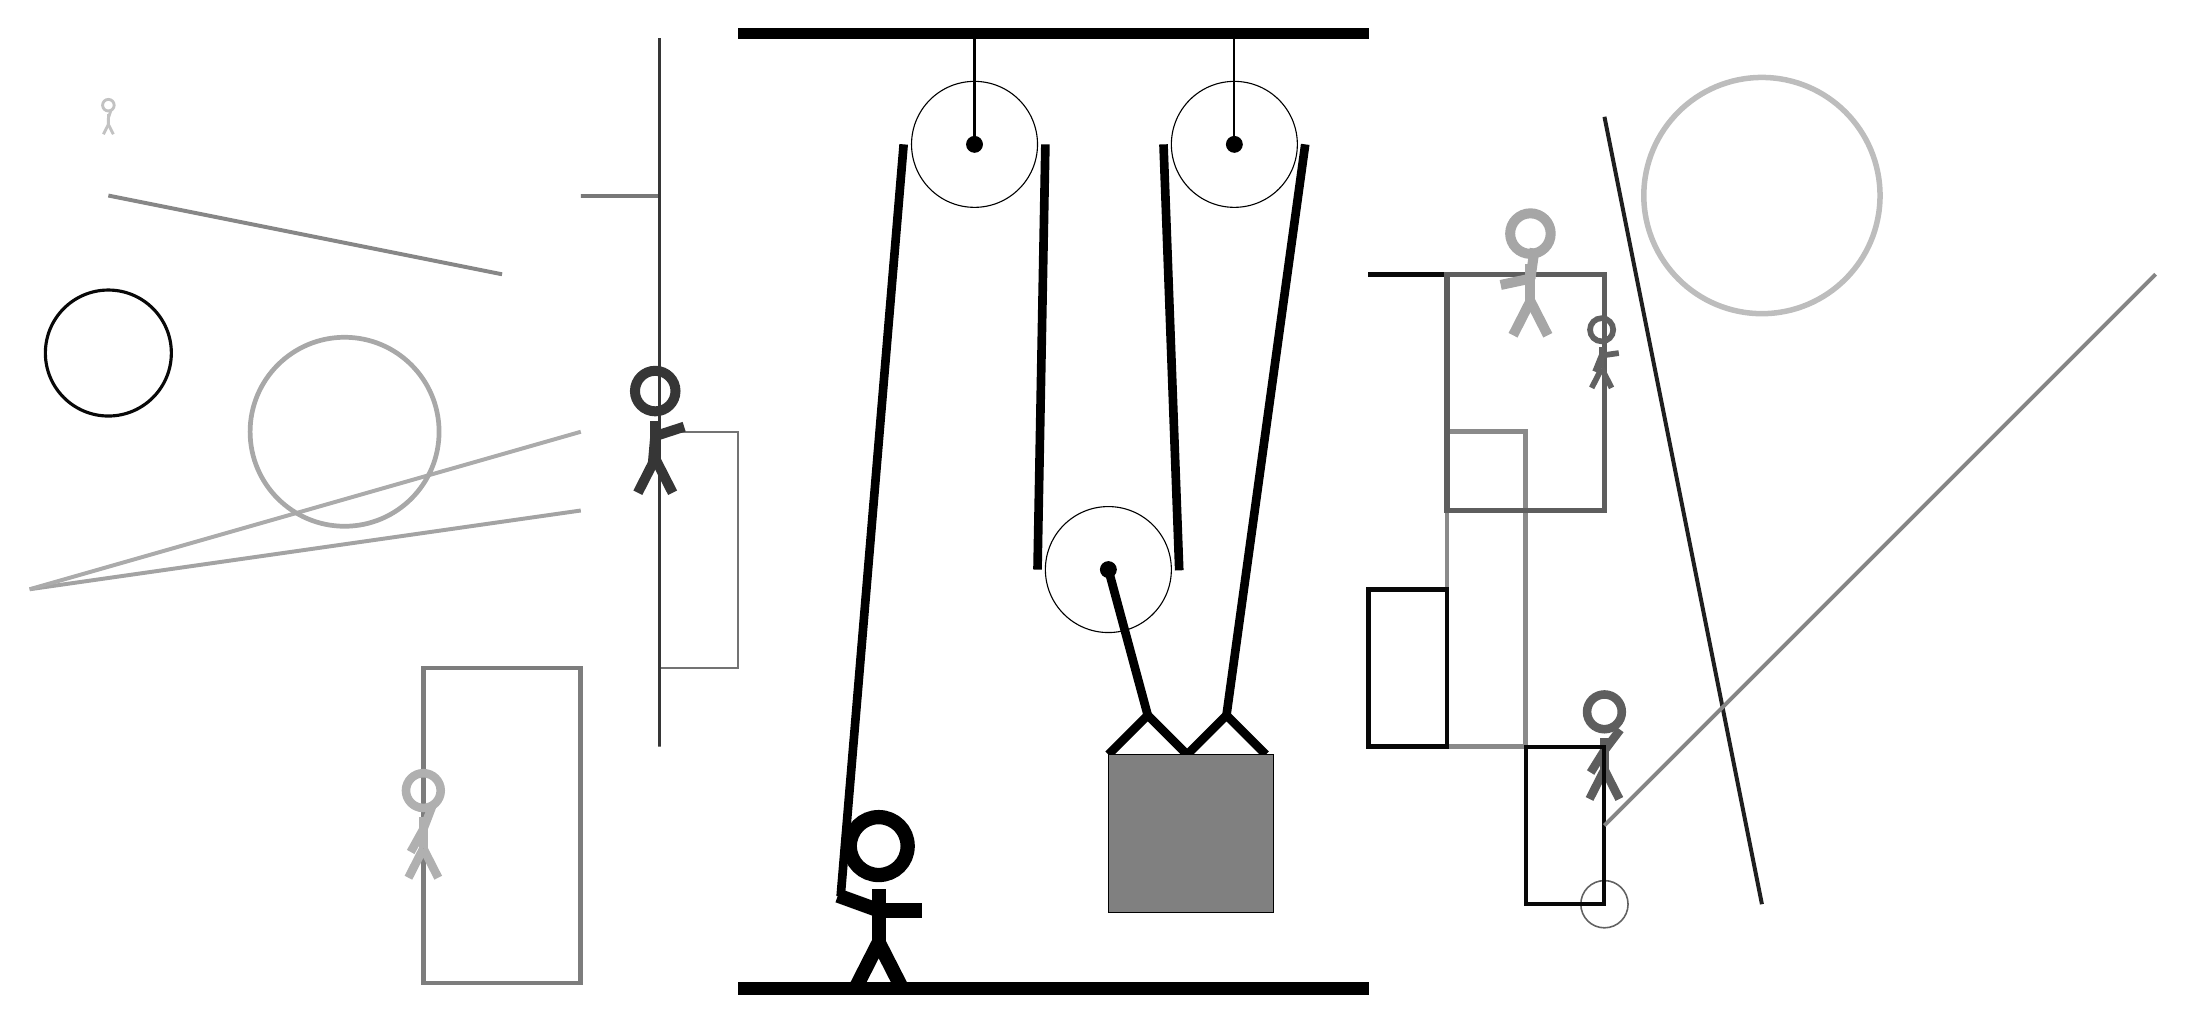
\begin{tikzpicture}
			%%%%% START %%%%%
			
			\draw[fill=black] (-2, 9) rectangle (6, 9.125);
			
			\draw[line width=0.6mm, color=black!51] (-4, -3) rectangle (-6, 1);
			
			\draw[line width=0.7mm, color=black!96] (8, 6) rectangle (6, 6);
			\draw[line width=0.5mm, color=black!53] (-4, 7) rectangle (-3, 7);
			\draw[line width=0.3mm, color=black!55] (-2, 4) rectangle (-3, 1);
			\draw[line width=0.5mm, color=black!36](-4, 3) -- (-11, 2);
			
			\draw[line width=0.5mm, color=black!33](-4, 4) -- (-11, 2);
			\draw [line width=0.2mm, color=black!62](9, -2) circle (0.3);
			\node[line width=0.3mm, color=black!31] at (-6, -1) {\Strichmaxerl[6][61][69]};
			\draw[line width=0.3mm, color=black!79] (-3, 0) rectangle (-3, 9);
			\draw[line width=0.5mm, color=black!47](-5, 6) -- (-10, 7);
			\node[line width=0.4mm, color=black!79] at (-3, 4) {\Strichmaxerl[7][85][18]};
			\draw[line width=0.6mm, color=black!46] (8, 0) rectangle (7, 4);
			\draw[line width=0.7mm, color=black!63] (7, 3) rectangle (9, 6);
			\node[line width=0.4mm, color=black!24] at (-10, 8) {\Strichmaxerl[2][89][72]};
			\draw [line width=0.4mm, color=black!97](-10, 5) circle (0.8);
			\node[line width=0.4mm, color=black!63] at (9, 0) {\Strichmaxerl[6][58][53]};
			
			\draw[line width=0.5mm, color=black!88](9, 8) -- (11, -2);
			\node[line width=0.7mm, color=black!62] at (9, 5) {\Strichmaxerl[4][68][8]};
			\draw [line width=0.7mm, color=black!26](11, 7) circle (1.5);
			\draw[line width=0.6mm, color=black!97] (7, 0) rectangle (6, 2);
			\draw [line width=0.6mm, color=black!34](-7, 4) circle (1.2);
			
			\node[line width=0.2mm, color=black!35] at (8, 6) {\Strichmaxerl[7][12][82]};
			
			\draw[line width=0.5mm, color=black!97] (8, -2) rectangle (9, 0);
			\draw[line width=0.5mm, color=black!48](9, -1) -- (16, 6);
			
			\draw (1, 7.65) circle (0.8);
			\draw[fill=black] (1, 7.65) circle (0.1);
			\draw[thick] (1, 7.65) -- (1, 9);
			
			\draw (4.3, 7.65) circle (0.8);
			\draw[fill=black] (4.3, 7.65) circle (0.1);
			\draw[thick] (4.3, 7.65) -- (4.3, 9);
			
			\draw (2.7, 2.25) circle (0.8);
			\draw[fill=black] (2.7, 2.25) circle (0.1);
			
			\draw[line width=1.1mm]  (2.7, -0.1) -- (3.2, 0.4) -- (3.7, -0.1) -- (4.2, 0.4) -- (4.7, -0.1);
			\draw[fill=black!50] (2.7, -0.1) rectangle (4.8, -2.1);
			
			\draw[line width=1.1mm](-0.7, -1.9) -- (0.1, 7.65);
			\centerarc[line width=1.1mm](1, 7.65)(0:180:0.9);
			\draw[line width=1.1mm](1.9, 7.65) -- (1.8, 2.25);
			\centerarc[line width=1.1mm](2.7, 2.25)(180:370:0.9);
			\draw[line width=1.1mm] (3.6, 2.24) -- (3.4, 7.65);
			\centerarc[line width=1.1mm](4.3, 7.65)(0:180:0.9);
			\draw[line width=1.1mm](4.2, 0.4) -- (5.2, 7.65);
			\draw[line width=1.1mm] (3.2, 0.4) -- (2.7, 2.25);
			
			\node at (-0.2, -2) {\Strichmaxerl[10][-20][0]};
			
			\draw[fill=black] (-2, -3) rectangle (6, -3.15);
			
			%%%%% END %%%%%
		\end{tikzpicture}
	\end{figure}	
\end{document}